\section{Excitations on the momentum--energy plane}\label{sec:9.3}

At $q = \SI{50}{keV}$ and $\omega = \SI{50}{meV}$ silicon has phonon final states and nothing else. At \SI{1}{keV} and \SI{1.3}{eV} its one final state is an electron--hole pair together with a phonon; at \SI{1}{keV} and \SI{3}{eV} a pair without a phonon is open as well. Each excitation in the atlas of \cref{tab:9-atlas} has a \emph{support}, the region of the $(q,\omega)$ plane where its response $S(\vect{q},\omega)$ of \cref{sec:4.2} carries weight. Where the support is formally unbounded, as for the multiphonon tails of \cref{sec:5.6}, we draw the region that holds \SI{90}{\percent} of the weight. \Cref{fig:9-qomega} draws the supports of silicon on the axes of \cref{fig:1-kinematics}, each in the color of its sector of \cref{eq:8.6-partition}. Where two supports overlap, a rate can count a final state twice, or drop an interference term, and the decomposition theorem of \cref{sec:8.6} decides which of the two dangers is real.

\subsection{The silicon plane by sector}\label{sec:9.3-silicon}

\begin{figure}[tbp]
  \centering
  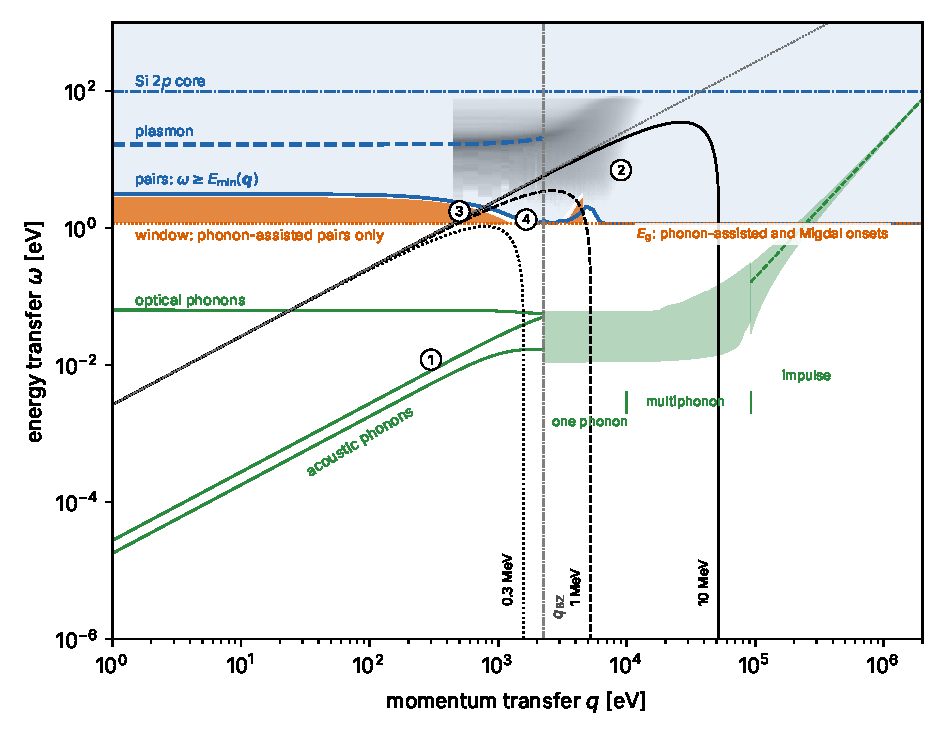
\includegraphics[width=\linewidth]{figures/ch09/fig9_2.pdf}
  \caption{The excitations of silicon on the plane of momentum transfer $q$ and energy deposited $\omega$, on the axes of \cref{fig:1-kinematics}. Green, electron-following sector: the transverse and longitudinal acoustic branches and the optical branch along [100] inside the zone, from the PBE force constants of \cref{sec:5.2}; beyond the zone radius $q_{\mathrm{BZ}} = \SI{2.25}{keV}$ (dash-dotted), the band holding the central \SI{90}{\percent} of the weight that creates phonons (5 and \SI{95}{\percent} quantiles), in the incoherent harmonic response at $T = 0$ with the PBE density of states, and above \SI{92.5}{keV} the same quantiles of the impulse Gaussian about the free recoil $q^2/2M$ (dashed); ticks at \SI{10}{keV} and \SI{92.5}{keV} separate the one-phonon, multiphonon and impulse regimes. Blue, zero-phonon electronic sector: the pair continuum above $E_{\mathrm{min}}(\vect{q})$, drawn as the lowest of the PBE edges along [100], [110] and [111] with the conduction bands shifted to the measured gap $\Eg = \SI{1.17}{eV}$, and as $\Eg$ beyond \SI{6.5}{keV}; gray scale, the random-phase loss function with local fields of the tables of Knapen, Kozaczuk and Lin~\cite{knapen2021dark} (scissor to the gap of \SI{1.17}{eV}, directions averaged, \num{e-3} to 4 on a logarithmic scale); dashed, the plasmon of the valence electron gas, $\omega_{\mathrm{pl}}^2 = \omega_p^2 + \tfrac35q^2v_{\mathrm{F}}^2$ with $\omega_p = \SI{16.6}{eV}$, up to \SI{2.24}{keV}, where this dispersion meets the pair continuum; dash-dotted, the $2p$ core level at \SI{99.4}{eV}. Orange, phonon-dressed electronic sector: the off-shell window along [100], from the phonon-assisted onset $\Eg + \omega_{\mathrm{TA}}$ up to $E_{\mathrm{min}} - \delta_{\mathrm{w}}$ with $\delta_{\mathrm{w}} = \SI{0.3}{eV}$; white above it, the margin of width $\delta_{\mathrm{w}}$ below the edge; dotted, $\Eg$, above which phonon-assisted pairs and Migdal events exist at every $q$. Black: the largest energy deposited, $qv_{\mathrm{max}} - q^2/2\mchi$, for $\mchi = 0.3$ (dotted), 1 (dashed) and \SI{10}{MeV} (solid), and $qv_{\mathrm{max}}$ (gray dotted), with $v_{\mathrm{max}} = 2.650\times10^{-3}$. Circled numbers mark the interference terms of \cref{tab:9-overlaps}.}
  \label{fig:9-qomega}
\end{figure}

\paragraph{Electron-following sector.} Inside the zone the support is a set of lines, the phonon branches of \cref{sec:5.2}. The acoustic branches rise as $\omega = c_\nu q$ from the origin and flatten at the zone boundary, at \SI{17}{meV} (transverse) and \SI{51}{meV} (longitudinal) at X in the PBE calculation; the optical branch stays near \SI{64}{meV}. Beyond the zone nothing new appears in energy. The momentum transfer is never folded (\cref{sec:1.3}); the nucleus keeps $\vect{q}$, and the phonon carries $\vect{q}$ minus a reciprocal-lattice vector. A single phonon therefore has energies between zero and \SI{64}{meV} at every $q$, and its weight changes as the Debye--Waller exponent $2W_\kappa = q^2\langle u_x^2\rangle$ of \cref{eq:5.6-W} grows. The PBE density of states of \cref{sec:5.2} gives $\langle u_x^2\rangle = \SI{2.45e-3}{\angstrom^2}$ at $T = 0$, so $2W_\kappa = 0.016$ at \SI{5}{keV}, 0.063 at \SI{10}{keV} and 1.0 at \SI{40}{keV}. Two and more phonons fill the band as $2W_\kappa$ approaches one. In the incoherent approximation the central \SI{90}{\percent} of the weight that creates phonons lies between 11 and \SI{60}{meV} at the zone radius $q_{\mathrm{BZ}} = \SI{2.25}{keV}$, still the one-phonon band. It lies between 13 and \SI{129}{meV} at \SI{46}{keV}, where the recoil parameter $x_R$ of \cref{eq:8.5-xR} is one, and between 46 and \SI{311}{meV} at \SI{92.5}{keV}. At that momentum the impulse approximation of \cref{sec:11.4} takes over from the sum over phonon numbers. It treats the nucleus as kicked so hard that its spectrum is a Gaussian of width $(E_R\langle\omega\rangle)^{1/2}$ about the free recoil energy $E_R = q^2/2M$, with $\langle\omega\rangle = \SI{40.9}{meV}$ the mean phonon energy. From there on the support is a band that follows $q^2/2M$ and narrows in relative width as $x_R^{-1/2}$.

The free recoil line crosses the gap at $q = (2M\Eg)^{1/2} = \SI{247}{keV}$, and the upper edge of the band does so at \SI{212}{keV}. Above these momenta electron-following final states sit at the same $(q,\omega)$ as electronic ones. A particle must be heavier than \SI{46.8}{MeV} to supply \SI{247}{keV}.

\paragraph{Zero-phonon electronic sector.} An electron--hole pair with no net phonon must take the whole momentum transfer itself, and its support is the continuum $\omega \ge E_{\mathrm{min}}(\vect{q})$ of \cref{eq:3.3-Emin}. With the bands of \cref{fig:3-si-bands}, shifted to the measured indirect gap, the edge lies at \SI{3.17}{eV} for $q \to 0$, at \SI{1.77}{eV} at \SI{1}{keV} along the lowest of the three symmetry directions, and reaches $\Eg = \SI{1.17}{eV}$ at the valley momentum $k_{\mathrm{c}} = \SI{1.94}{keV}$. The value at $q \to 0$ lies below the measured direct gap of \SI{3.4}{eV}, because a shift fitted to the indirect gap does not correct the vertical gap at $\mathrm{\Gamma}$ (\cref{sec:3.3}). At larger $|\vect{q}|$ the edge depends on the direction of $\vect{q}$. It returns to $\Eg$ whenever $\vect{q}$ equals a valley momentum plus a reciprocal-lattice vector, $\vect{k}_{\mathrm{c}} + \vect{G}$, whose lengths are 1.94, 2.63, 3.25, 4.96, 5.27, \SI{5.32}{keV} and so on. Above \SI{6.4}{keV} they leave no gap wider than \SI{0.72}{keV}, and half that distance costs a pair of mass $1.19\,m_e$ about \SI{0.11}{eV} above $\Eg$. There the onset of the direction average that enters an isotropic rate stays within about a tenth of an eV of the gap. Below, the widest gap lies between 3.25 and \SI{4.96}{keV}; there the lowest of the three symmetry-line edges rises to \SI{2.07}{eV}, an upper value for the onset over all directions. Upward the continuum is unbounded. At small $q$ its weight sits at the absorption peaks of 3.4 and \SI{4.2}{eV} and in the plasmon; at large $q$ it concentrates along the free-electron recoil $q^2/2m_e$, the ridge of the gray scale in \cref{fig:9-qomega}.

The plasmon, the exciton and the core shells lie inside this region and have homes of their own. The plasmon of \cref{sec:4.5} starts at the measured loss peak of \SI{16.4}{eV}, \SI{0.2}{eV} below the $\omega_p = \SI{16.6}{eV}$ of the valence electron gas, and disperses upward. With the quadratic dispersion of the gas it is a line up to \SI{2.24}{keV}, where it enters the pair continuum and Landau damping removes its weight; the exact zero of the Lindhard function enters at $q_{\mathrm{c}} = \SI{2.60}{keV}$ (\cref{sec:4.5}). In the loss-function tables that \cref{sec:10.2} uses, the peak moves from \SI{18.9}{eV} at \SI{0.5}{keV} to \SI{22.3}{eV} at \SI{2.45}{keV}; the small-$q$ peak lies \SI{2.5}{eV} above the measured \SI{16.4}{eV} because of the shift that sets their gap (\cref{sec:10.3}, which computes the plasmon's share of the rate). The bound pair, the exciton of \cref{sec:4.9}, lies \SI{14.7}{meV} below the edge near $q = k_{\mathrm{c}}$; on the scale of the figure it coincides with the edge (\cref{sec:10.5}, the exciton lines at finite momentum). The core shells start at fixed energies, \SI{99.4}{eV} for $2p$ and \SI{150}{eV} for $2s$, and carry weight at momentum transfers of tens of keV, the momenta of the electrons in them (\cref{sec:10.6}).

\paragraph{Phonon-dressed electronic sector.} A pair created together with a phonon needs no particular momentum, because the phonon carries whatever crystal momentum the pair lacks. Its support starts just above the gap at every $q$, at the onset $E^{\mathrm{PA}}_{\mathrm{min}}(\vect{q}) = \Eg + \omega_{\mathrm{TA}}(\vect{k}_{\mathrm{c}} - \vect{q})$ of \cref{eq:13.1-EPA}, and never above $\Eg + \SI{64}{meV} = \SI{1.23}{eV}$. With the PBE force constants the onset is \SI{1.187}{eV} at $q \to 0$ and \SI{1.184}{eV} at \SI{1}{keV}. Between this onset and the zero-phonon edge lies the \emph{off-shell window} of \cref{sec:8.6}, the region below $E_{\mathrm{min}}(\vect{q}) - \delta_{\mathrm{w}}$ where no zero-phonon pair exists and every electronic final state carries a phonon. Along the valley axis, with $\delta_{\mathrm{w}} = \SI{0.3}{eV}$, it spans 1.184 to \SI{1.467}{eV} at \SI{1}{keV} and closes at \SI{1.27}{keV} with the computed bands. It reopens beyond \SI{3.30}{keV}, on the far side of the Umklapp image of the opposite valley (\cref{sec:13.6}, which fixes the margin and the window edges). Above the zero-phonon edge the same sector is the phonon sideband of the zero-phonon continuum, and there it is a correction to the zero-phonon rate (\cref{sec:13.9} compares the two).

The Migdal effect of a nucleon coupling, which straddles the two electronic sectors (\cref{sec:9.1-sectors}), has the same support. The struck nucleus absorbs the momentum and the electrons take an energy $\omega_e \ge \Eg$, at every $q$. What separates it from a pair made through the electron density is the operator, not the region of the plane.

\subsection{Overlap regions and interference}\label{sec:9.3-overlap}

One phonon and two phonons share the band below \SI{64}{meV}. The impulse band and the pair continuum share the region above \SI{212}{keV} and \SI{1.17}{eV}, and the phonon sideband and the zero-phonon continuum share everything above $E_{\mathrm{min}}(\vect{q})$. An overlap in the plane is not by itself an interference. Sectors add (\cref{sec:9.1-sectors}), to the accuracy of the leak in \cref{eq:8.6-decomp}, and within one sector so do different phonon numbers: one and two phonons are orthogonal final states, and so are a nucleus recoiling with the electrons in their ground state and a pair. Interference needs two amplitudes into the same final state, and on the silicon plane that happens in two ways. The first is a coupling to both species, as for a dark photon, whose cross terms $S_{e\kappa}$ fill the bottom row of \cref{tab:8-sectors} and are derived, with their sizes, in \cref{sec:17.4}. The second is the boundary between the two electronic sectors, within $\delta_{\mathrm{w}}$ below the zero-phonon edge and a few pair widths above it. Only the sum $S^0 + S^+$ is defined there, the Dyson convention \cref{eq:8.6-dyson} splits it, and the decay of a zero-phonon pair can interfere with the same one-phonon state made directly, the Fano term \cref{eq:8.6-fano}. Inside that margin only totals of the two electronic sectors are quoted (\cref{sec:13.6}).

\subsection{The kinematic reach on the plane}\label{sec:9.3-reach}

Particles of mass $\mchi$ reach the region below $\omega = qv_{\mathrm{max}} - q^2/2\mchi$ (\cref{eq:1.3-region}), and the black curves of \cref{fig:9-qomega} show it for three masses. A particle of \SI{0.3}{MeV} deposits at most \SI{1.05}{eV}, at $q = \SI{0.80}{keV}$, and transfers at most \SI{1.59}{keV}. Its region lies below the gap and inside the zone, so it meets single acoustic and optical phonons and nothing else, with $2W_\kappa \le 0.002$. A particle of \SI{1}{MeV} deposits at most \SI{3.51}{eV} and crosses the gap for momentum transfers between 0.49 and \SI{4.81}{keV}. It enters the off-shell window, where every pair it makes carries a phonon, and the zero-phonon continuum above the edge, while its lattice final states are still single phonons ($2W_\kappa \le 0.018$ at its largest $q$, \SI{5.3}{keV}). A particle of \SI{10}{MeV} transfers up to \SI{53}{keV}, where $2W_\kappa = 1.8$, and reaches deep into the multiphonon band. In energy it reaches \SI{35}{eV}, across the region of the plasmon, but not the plasmon line, which ends at \SI{2.24}{keV}, where this particle deposits no more than \SI{5.9}{eV}; nor the $2p$ shell at \SI{99.4}{eV}, nor the impulse band, which opens at \SI{17.5}{MeV}. The lightest mass whose curve touches a region is the lightest mass of that channel (\cref{sec:9.2}).

\begin{workedexample}{The excitations open at 5 keV and 2 eV in silicon}\label{we:9-open}
Take $q = |\vect{q}| = \SI{5}{keV}$ and $\omega = \SI{2}{eV}$. The point is reachable if $qv_{\mathrm{max}} - q^2/2\mchi \ge \omega$, with $qv_{\mathrm{max}} = \SI{13.25}{eV}$, that is for $\mchi \ge q^2/[2(qv_{\mathrm{max}} - \omega)] = \SI{1.11}{MeV}$; at \SI{10}{MeV} the minimum speed of \cref{eq:1.3-vmin} is $\vmin = \omega/q + q/2\mchi = 6.50\times10^{-4}$, or \SI{195}{km.s^{-1}}, well inside the halo.

\emph{Electron-following.} At \SI{5}{keV}, $2W_\kappa = 0.016$ and $E_R = \SI{0.48}{meV}$. Two electronvolts would take at least 32 phonons of \SI{64}{meV}, each costing a factor of order $2W_\kappa$ in weight. The sector is closed.

\emph{Zero-phonon electronic.} The edge depends on the direction of $\vect{q}$. Along [100], [110] and [111] it lies at 2.59, 2.02 and \SI{2.31}{eV}, all above \SI{2}{eV}: along the symmetry lines no pair without a phonon exists at this point. But a valley image $\vect{k}_{\mathrm{c}} + \vect{G}$ has length \SI{4.96}{keV}, and for $\vect{q}$ near that direction the pair costs $\Eg$ plus about \SI{1}{meV}. Averaged over directions the zero-phonon response is thus open, but small: the direction-averaged loss function of the tables of \cref{sec:10.2} at this $q$ is \num{8.8e-4} at \SI{2}{eV}, against its maximum of 0.33 at \SI{35.7}{eV}. The plasmon line has ended at \SI{2.24}{keV}, the exciton lies \SI{14.7}{meV} below the edge, and the $2p$ shell needs \SI{99.4}{eV}: none of them is open.

\emph{Phonon-dressed electronic.} The phonon-assisted onset lies below \SI{1.23}{eV} for every $\vect{q}$, so phonon-assisted pairs are open. Where the point sits relative to the zero-phonon edge again depends on direction. Along [100] it lies below $E_{\mathrm{min}} - \delta_{\mathrm{w}} = \SI{2.29}{eV}$, inside the window, and phonon-assisted pairs are the one electronic final state there. Along [111] it lies inside the window by \SI{11}{meV} ($E_{\mathrm{min}} - \delta_{\mathrm{w}} = \SI{2.011}{eV}$), less than the exciton binding and less than the difference between a symmetry-line edge and the minimum over all crystal momenta. Along [110] it lies in the margin, between 1.72 and \SI{2.02}{eV}, where only the total of the two electronic sectors is defined. A nucleon coupling reaches the same final states through the Migdal effect, with a probability per scattering of order $(E_R/\langle\omega_e\rangle)(\delta M_\kappa/M_\kappa) = 2\times10^{-8}$ by the moment estimate of \cref{sec:12.1}. Here $\langle\omega_e\rangle \approx \SI{6}{eV}$ is the mean electronic excitation energy, and $\delta M_\kappa/M_\kappa = Z_\kappa m_e/M_\kappa = 2.7\times10^{-4}$ the share of the atom's mass carried by the electrons that move with the nucleus (\cref{sec:8.6}).

\emph{Interference.} For a dark photon the cross cells of regions 2 and 3 of \cref{tab:9-overlaps} are both present, each a few parts in $10^4$ of its sector, and for directions in the margin the Fano term of region 4 vanishes in silicon. The point is thus served by two sectors in different directions of $\vect{q}$, which is why a calculation applies the window bin by bin in $(|\vect{q}|,\hat{\vect{q}})$ and not to the direction average (\cref{sec:13.6}).
\end{workedexample}

\subsection{Supports in other materials}\label{sec:9.3-others}

The remaining rows of the atlas belong to other materials, and their supports reduce to a few shapes: a dispersing line, a flat line at a fixed energy, a continuum above a threshold, or a point at $q \to 0$. \Cref{tab:9-supports} gives the shape and one number for each, with the section that treats it. Absorption samples the single point of \cref{eq:9.2-abs}, far to the left of every scattering curve, and a support absorbs if it reaches $q \to 0$ at that energy (\cref{sec:9.1-empty}).

\begin{table}[tbp]
  \centering
  \small
  \caption{Supports in the $(q,\omega)$ plane of the excitations of the atlas that silicon does not have, with one characteristic number for the material that the treating section uses. ``Line'' means one energy for each $q$; ``continuum'' a band of energies at each $q$. $g_{33}$: component of the gyration tensor along the optic axis; $g_c$: Luttinger charge parameter of a one-dimensional metal.}
  \label{tab:9-supports}
  \begin{tabular}{@{}p{0.24\linewidth}p{0.32\linewidth}p{0.23\linewidth}p{0.10\linewidth}@{}}
    \toprule
    Excitation & Support & Scale & Home \\
    \midrule
    Optical phonons of polar crystals & line at $\omega_{\mathrm{L}}$ as $q \to 0$, reached by a coupling to charge & GaAs \SI{36.35}{meV} & \cref{sec:11.2} \\
    Phonons of a quantum crystal & acoustic lines and multiphonon band of a light, strongly anharmonic lattice & solid helium, below \SI{3}{meV} at low pressure & \cref{sec:11.5} \\
    Magnons & line from an anisotropy gap at the zone center to the top of the band & NiO, gap \SI{4.54}{meV} (measured; anisotropy added to the model), top \SI{118}{meV} & \cref{sec:14.1} \\
    Two-magnon continua & continuum from the one-magnon energy to twice the band top at small $q$ & NiO, up to \SI{236}{meV} & \cref{sec:14.2} \\
    Chiral and nonreciprocal modes & the supports above; the response acquires a part odd in $\vect{q}$ & $\alpha$-quartz, $q\,g_{33} = 7\times10^{-5}$ at \SI{2.1}{eV} & \cref{sec:14.5} \\
    Precessing nuclear spins & point at $q \to 0$, $\omega$ at the Larmor frequency & $^{207}$Pb in \SI{26.8}{mT}: \SI{241.8}{kHz} (\SI{1}{neV}) & \cref{sec:14.6} \\
    Superconducting quasiparticle pairs & continuum $\omega \ge 2\Delta_{\mathrm{BCS}}$ inside the particle--hole band $\omega \le qv_{\mathrm{F}} + q^2/2m_e$ of the metal & aluminum, $2\Delta_{\mathrm{BCS}} = \SI{0.36}{meV}$ & \cref{sec:15.1} \\
    Dirac and narrow-gap pairs & continuum $\omega \ge (4\Delta_{\mathrm{D}}^2 + v_{\mathrm{D}}^2q^2)^{1/2}$ & ZrTe$_5$, $\Delta_{\mathrm{D}} = \SI{11.8}{meV}$ & \cref{sec:16.1} \\
    Low-dimensional plasmons & line $\omega \propto q_\parallel$, faster than the halo, reached by oblique $\vect{q}$ & metallic nanotube, $\omega = v_{\mathrm{D}}q_\parallel/g_c$, 3.4 to 6.9 times $v_{\mathrm{max}}$ & \cref{sec:16.2} \\
    Graphene, nanotubes, quantum dots & continuum above a confinement gap; ejection above the work function & PbS dot \SI{1.2}{eV}; graphene \SI{4.3}{eV} & \cref{sec:16.3} \\
    Molecular (Frenkel) excitons & nearly flat lines at molecular energies & anthracene \SI{3.1}{eV} & \cref{sec:16.4} \\
    Dopant transitions & flat lines and an ionization continuum & Si:P, binding \SI{45.59}{meV} & \cref{sec:16.5} \\
    Color centers, broken bonds & reached through a nuclear recoil above a displacement or bond energy & H$_2$ bond \SI{4.75}{eV}; displacement tens of eV & \cref{sec:16.6} \\
    Two-level systems in glasses & flat continuum of splittings, independent of $q$ & down to \si{\micro eV}; \SI{e20}{eV^{-1}.cm^{-3}} & \cref{sec:16.7} \\
    Bulk acoustic modes of a body & points at $q \to 0$, the normal modes of the whole detector & MHz (mm crystal) to kHz (ton-scale bar) & \cref{sec:11.8} \\
    \bottomrule
  \end{tabular}
\end{table}

For superconductors and Dirac materials the sectors are those of quasiparticle number (\cref{sec:9.1-sectors}), so the rules of \cref{sec:9.3-overlap} for which overlaps add and which interfere hold only as far as those sectors are defined, which \cref{sec:8.6} bounds but does not settle.
